\subsection{Executable Packing}
\begin{frame}
    \frametitle{Binary Protection}
    \begin{itemize}
        \item Malware authors use both packers and crypters to reduce file size and increase analysis time
        \item Packers confuse disassembly by making code look like data
        \item A packer may contain anti-debugger/disassembler tricks such as SEH trickery and jumping into the middle of instructions
        \item A number of packers exist
            \pedbullet{PE: UPX, ASPack, tElock, yodacrypt, FSG, etc...}
            \pedbullet{ELF: UPX, BurnEye, etc...}
        \item We will create a basic packer to gain a better understanding of unpacking
    \end{itemize}
\end{frame}

\begin{frame}
    \frametitle{Packer Components}
    \begin{itemize}
        \item The original executable code of the target application must be obfuscated or encrypted
        \item When the application is launched the packer decoder routine must be executed first (entry point modification)
        \item The decoder routine must restore the original executable code
        \item The decoder routine must transfer control to the original executable code
        \item To get a better understanding of this subject we're going to manually construct a packer
    \end{itemize}
\end{frame}

\begin{frame}
    \frametitle{What Packing is Not}
    \begin{itemize}
        \item We don't consider run-time instrumented protection "packing"
            \pedbullet{Shiva}
        \item Such protection schemes do exist, but are rarely used in malware
            \pedbullet{Probably because they require compile time modifications}
    \end{itemize}
\end{frame}

\begin{frame}
    \frametitle{The Target Application}
    \begin{itemize}
        \item original\_hello.exe
            \pedbullet{Simple application written in C}
            \pedbullet{Prints "Hello World" and waits for keypress}
        \item Examine the PE structure information of the original executable:
    \end{itemize}
    \begin{center}
        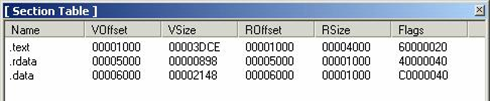
\includegraphics[scale=.50]{images/executable_packing/the_target_application.png} \\
    \end{center}
    \begin{itemize}
        \item Notice the virtual size of 0x3DCE and the raw size of 0x4000 indicating that there should be 562 bytes of slack space at the end of the .TEXT section
        \item Verify this fact with a hex editor (offset 0x4DCE)
    \end{itemize}
\end{frame}

\begin{frame}
    \frametitle{Abusing Slack Space}
    \begin{itemize}
        \item We are going to take advantage of the identified slack space by inserting our decoder stub into it
        \item PE modifications must be made
            \pedbullet{The .TEXT section must be made writable so our decoder stub can modify it}
            \pedbullet{The VSize must be increased so our decoder stub gets mapped into memory}
    \end{itemize}
    \begin{center}
        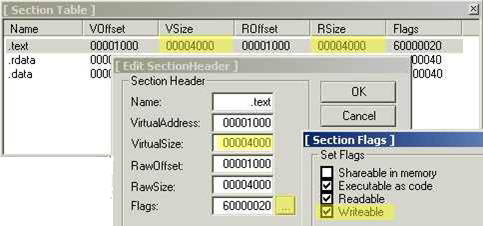
\includegraphics[scale=.40]{images/executable_packing/abusing_slack_space.png} \\
    \end{center}
\end{frame}

\begin{frame}
    \frametitle{Abusing Slack Space}
    \begin{itemize}
        \item Next, we must modify the Entry Point (EP) to point to our decoder stub. Lets set it to 0x4E00
        \item Alternative strategies for storing a decoder stub include
            \pedbullet{New sections}
            \pedbullet{Instruction gap abuse}
            \pedbullet{Entirely new PE file}
    \end{itemize}
\end{frame}

\begin{frame}[fragile]
    \frametitle{Encoding the Executable Code}
    \begin{itemize}
        \item For the purposes of this exercise we will manually encode the original executable code
        \item Simple XOR routine (VB):
    \end{itemize}
    \begin{tiny}
    \begin{semiverbatim}
        StartAt = &H1048   'Original EP
        length  = &H2D86   '3DCE - 1048 (Original VSize � Original EP)

        Open filename For Binary As file

        For i = 1 To length
            offset = StartAt + i
            Get file, offset, byte
            byte = byte Xor &HF
            Put file, offset, byte
        Next

        Close file
    \end{semiverbatim}
    \end{tiny}
    \begin{itemize}
        \item Compiled helper app: do\_opcode\_crypt.exe
    \end{itemize}
\end{frame}

\begin{frame}[fragile]
    \frametitle{Writing the Decoder Stub}
    \begin{itemize}
        \item Our binary is now ready to accept a decoder
        \item We'll write the decoder in C, compile it and then extract the byte code
    \end{itemize}
    \begin{tiny}
    \begin{semiverbatim}
        void main (void)
        \{
            int i;
            char b;

            char *buffer = 0x400000;   // imagebase
            long length  = 0xBEEF;     // length of code (placeholder)

            buffer += 0xDEAD;          // OEP offset (placeholder)

            for(i = 0; i < length; i++)
            \{
                b = buffer[i];
                b = b ^ 0xF;
                buffer[i] = b;
            \}

            _asm jmp buffer
        \}
    \end{semiverbatim}
    \end{tiny}
\end{frame}

\begin{frame}[fragile]
    \frametitle{Converting the Decoder Stub}
    \begin{itemize}
        \item Compile the decoder stub in Visual C
        \item Set a breakpoint at the top of the code
        \item Enter the debugger with F5 and choose �goto disassembly�
        \item Disassembly excerpt:
    \end{itemize}
    \begin{tiny}
    \begin{semiverbatim}
        \alert{EB 09      }   jmp   main+43h
        \alert{8B 4D FC   }   mov   ecx, dword ptr [ebp-4]
        \alert{83 C1 01   }   add   ecx, 1
        \alert{89 4D FC   }   mov   dword ptr [ebp-4], ecx
        \alert{8B 55 FC   }   mov   edx, dword ptr [ebp-4]
        \alert{3B 55 F0   }   cmp   edx, dword ptr [ebp-10h]
        \alert{7D 22      }   jge   main+6Dh
        \alert{8B 45 F4   }   mov   eax, dword ptr [ebp-0Ch]
        \alert{03 45 FC   }   add   eax, dword ptr [ebp-4]
        \alert{8A 08      }   mov   cl, byte ptr [eax]
        \alert{88 4D F8   }   mov   byte ptr [ebp-8], cl
        \alert{0F BE 55 F8}   movsx edx, byte ptr [ebp-8]
    \end{semiverbatim}
    \end{tiny}
\end{frame}

\begin{frame}[fragile]
    \frametitle{Inserting the Decoder Stub}
    \begin{itemize}
        \item Copy out the hex bytes (\alert{remove newlines}):
    \end{itemize}
    \begin{tiny}
    \begin{semiverbatim}
        C745F400004000C745F0EFBE00008B45F405ADDE00008945F4C745FC
        00000000EB098B4DFC83C101894DFC8B55FC3B55F07D228B45F40345
        FC8A08884DF80FBE55F883F20F8855F88B45F40345FC8A4DF88808EB
        CDFF65F4
    \end{semiverbatim}
    \end{tiny}
    \begin{itemize}
        \item Open the target application in WinHex
        \item Highlight offset 0x4E00, hit Ctrl+B (write clipboard) and select �ASCII Hex�
        \item The final step is to modify the placeholders with real values. Remember, little endian
    \end{itemize}
    \begin{tiny}
    \begin{semiverbatim}
        Offset      0  1  2  3
        00004E10   .. .. AD DE    (DEAD)
        00004E10   .. .. 48 10    (1048)

        Offset      0  1  2  3  4  5  6  7  8  9  A  B
        00004E00   .. .. .. .. .. .. .. .. .. .. EF BE  (BEEF)
        00004E00   .. .. .. .. .. .. .. .. .. .. 86 2D  (2D86)
    \end{semiverbatim}
    \end{tiny}
\end{frame}

\begin{frame}[fragile]
    \frametitle{Watch it in Action}
    \begin{itemize}
        \item Load the modified file in OllyDbg
        \item Look at the original EP and verify that it's not recognized as executable code
        \item Set a breakpoint at the end of the decoder stub
    \end{itemize}
    \begin{tiny}
    \begin{semiverbatim}
        00404E53  EB CD    JMP SHORT final.00404E22
        00404E55  FF65 F4  \alert{JMP [EBP-C]}               ; final.00401048
    \end{semiverbatim}
    \end{tiny}
    \begin{itemize}
        \item Hit F9 to run through the decoder
        \item Look at the original EP again
            \pedbullet{Right click "Analysis$\rightarrow$Analyze code" (Ctrl-A)}
    \end{itemize}
\end{frame}

\begin{frame}
    \frametitle{Exercise}
    \begin{itemize}
        \item Create your own packer
        \item Follow these high-level steps:
            \pedbullet{Copy original\_hello.exe to pe\_modified\_hello.exe}
            \pedbullet{Modify pe\_modified\_hello.exe with LordPE}
            \pedbullet{Run do\_opcode\_crypt.exe to create crypted.exe}
            \pedbullet{Insert the decoder stub into crypted.exe}
            \pedbullet{Verify crypted.exe works}
            \pedbullet{Verify crypted.exe is indeed "crypted"}
        \item Some shortcuts were made for you
    \end{itemize}
\end{frame}


\subsection{Executable Unpacking}
\begin{frame}[fragile]
    \frametitle{Detecting Packed Executables}
    \begin{itemize}
        \item Entry Point (EP) lies outside of .TEXT section
        \item .TEXT section is writable
        \item Sections with 0 size
        \item Limited imports
        \item No strings
        \item Entropy (compressibility of bytes)
            \pedbullet{Ghetto check: compression}
    \end{itemize}
    \begin{tiny}
    \begin{semiverbatim}
        \$ cat calc.exe | gzip -v > /dev/null
         55.8%

        \$ cat calc-upx.exe | gzip -v > /dev/null
         24.9%

        \$ cat calc-aspack.exe | gzip -v > /dev/null
         25.2%
    \end{semiverbatim}
    \end{tiny}
\end{frame}

\begin{frame}
    \frametitle{The Easy Way: PEiD}
    \begin{itemize}
        \item Has a multitude of signatures (somewhat outdated)
        \item You can add your own (many publicly exist)
        \item Entropy detection
        \item Generic detection
        \item Generic unpacking with intelligent OEP detection
    \end{itemize}
    \begin{center}
        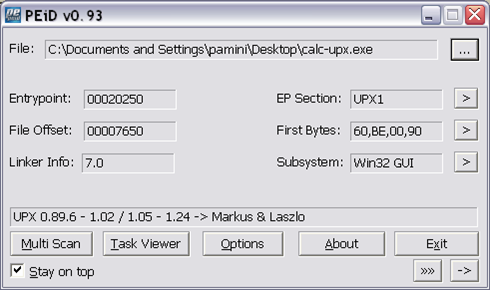
\includegraphics[scale=.50]{images/executable_packing/peid.png} \\
    \end{center}
\end{frame}

\begin{frame}
    \frametitle{Methodologies}
    \begin{itemize}
        \item There are three basic methodologies to unpacking
        \item Post execution analysis
            \pedbullet{An easy and generic approach}
            \pedbullet{Most dangerous}
        \item Controlled run-time analysis
            \pedbullet{More difficult to do}
            \pedbullet{More control / less dangerous}
            \pedbullet{PEiD attempts to automate this, but we don't trust anything automated}
        \item Static analysis / basic emulation
            \pedbullet{Most difficult to do}
            \pedbullet{Safe}
    \end{itemize}
\end{frame}

\begin{frame}
    \frametitle{Post Execution Analysis}
    \begin{itemize}
        \item Launch the packed binary in a controlled environment
        \item The decoder stub will run leaving an unpacked copy of the binary in memory
        \item Dump the running process to disk
            \pedbullet{OllyDbg +OllyDump}
            \pedbullet{ProcDump}
            \pedbullet{Etc...}
        \item Fix the Import Address Table (IAT) and analyze (more on this later)
    \end{itemize}
\end{frame}

\begin{frame}
    \frametitle{Controlled Run-Time Analysis}
    \begin{itemize}
        \item Load the packed binary in a debugger
        \item Single step through the decoder stub until a transfer is made to the Original Entry Point (OEP)
    \end{itemize}
    \begin{columns}
        \column{.5\textwidth}
            \begin{itemize}
                \item Dump the running process to disk
                    \pedbullet{OllyDbg +OllyDump}
                    \pedbullet{Etc...}
                \item Fix the Import Address Table (IAT) and analyze (more on this later)
            \end{itemize}
        \column{.5\textwidth}
            \begin{center}
                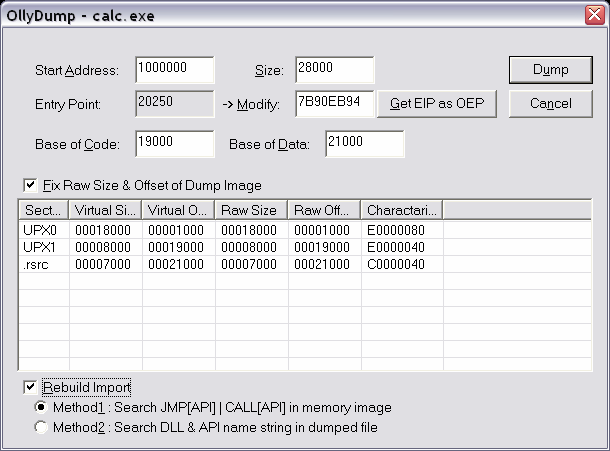
\includegraphics[scale=.50]{images/executable_packing/ollydump.png} \\
            \end{center}
    \end{columns}
\end{frame}

\begin{frame}
    \frametitle{IAT Reconstruction}
    \begin{itemize}
        \item Why do we want to rebuild the IAT?
            \pedbullet{Analyzing a malicious binary without symbols is burdensome}
        \item There are a number of approaches to IAT reconstruction
    \end{itemize}
    \begin{columns}
        \column{.5\textwidth}
            \begin{itemize}
                \item We will cover three approaches
                    \pedbullet{OllyDump}
                    \pedbullet{ImportRec}
                    \pedbullet{IDCDumpFix}
                \item Depending on the target, one approach may work better than another
            \end{itemize}
        \column{.5\textwidth}
            \begin{center}
                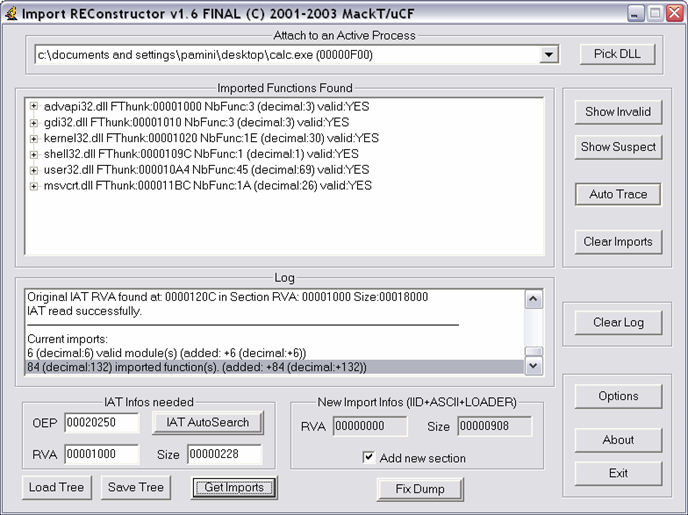
\includegraphics[scale=.50]{images/executable_packing/importrec.png} \\
            \end{center}
    \end{columns}
\end{frame}

\begin{frame}
    \frametitle{Static Analysis / Basic Emulation}
    \begin{columns}
        \column{.5\textwidth}
            \begin{itemize}
                \item If possible, such as with UPX, manually unpack the binary with the relevant unpacker
                \item Process the binary with an emulator such as Chris Eagle's x86-emu plug-in
                \item Single step through the decoder stub until the IDA database is completely decoded
            \end{itemize}
        \column{.5\textwidth}
            \begin{center}
                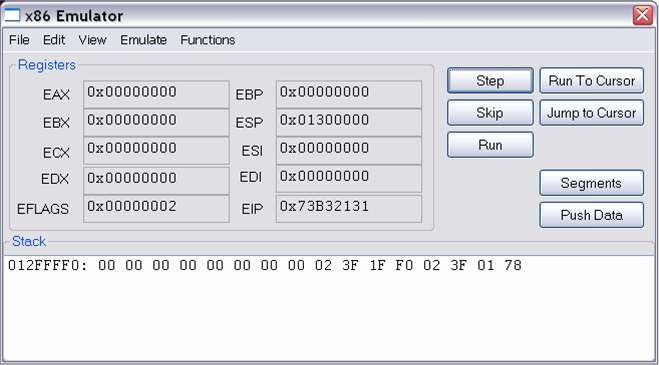
\includegraphics[scale=.50]{images/executable_packing/x86-emu.png} \\
            \end{center}
    \end{columns}
\end{frame}

\begin{frame}
    \frametitle{Exercises}
    \begin{itemize}
        \item Examine the PE structure of calc*.exe
        \item Unpack calc-aspack.exe using post execution analysis
        \item Unpack calc-upx.exe using controlled run-time analysis
        \item Unpack the custom packed file from the previous exercise using x86-emu
        \item For the daring, unpack calc-aspack.exe using controlled run-time analysis. Watch for the anti-disasm trickery at EP.
        \item Rebuild IATs using various techniques and compare.
        \item See the following files for hints ONLY if you get stuck
            \pedbullet{OpenRCE ASPack Notes.txt}
            \pedbullet{OpenRCE UPX Notes.txt}
    \end{itemize}
\end{frame}

\begin{frame}
    \frametitle{Automation Exercises}
    \begin{itemize}
        \item Automate the process of dumping and reconstruction with pydbg and pefile
        \item Attach to a running process
        \item Preprocess common system DLLs and harvest the default addresses of the exported symbols
        \item Scan and dump the address space while also looking for possible pointers to the DLL's exported symbols' addresses
        \item Generate IDAPython/IDC output that can be loaded directly into IDA to recover the symbols in the loaded dump
    \end{itemize}
\end{frame}


\begin{frame}
    \frametitle{Original Entry Point (OEP) Discovery Techniques}
    \begin{itemize}
        \item Graph analysis
        \item PUSH/POP trick
        \item Common APIs
        \item Markov chains on instruction patterns
        \item Taint analysis
    \end{itemize}
\end{frame}


\subsection{Packer Usage Statistics}
\begin{frame}
    \frametitle{The Corpus}
    \begin{itemize}
        \item Had just under 50.000 malware samples lying around
        \item Ran them through a beta of \emph{pefile} which employs \emph{PEiD}'s packer signature database
        \item In around 42\% of the files no packer could be found
        \item In the remaining (~58\%) of the files over 200 packers and compilers were identified
    \end{itemize}
\end{frame}

\begin{frame}
    \frametitle{Most Frequently Used}
    \begin{itemize}
        \item The most frequently occurring packer among the samples, \emph{UPX}, would probably not surprise anyone that has been looking at malware for a while.
        \item It appeared in around 13\% of the samples.
        \item \emph{Mew}, \emph{PeCompact}, \emph{ASPack}, \emph{FSG}, \emph{y0da's Crypter}, \emph{Armadillo} and other versions of UPX took the next places.
    \end{itemize}
\end{frame}

\begin{frame}
    \frametitle{Most Common Packers}
        \begin{center}
            \pgfimage[height=7cm]{images/executable_packing/packer_stats_pie_chart}
        \end{center}
\end{frame}


\begin{frame}
    \frametitle{The Long Tail}
    \begin{itemize}
        \item Reverse engineers and analysts have to confront a large variety of packers and their modified versions
        \item PEiD's largest databases have over 2000 entries
            \pedbullet{http://www.secretashell.com/BobSoft/}
        \item The most obscure packers tend to appear with a relatively low frequency
        \item Yet, it's usually those more exotic packers, the ones incorporating fancier techniques
        \item In the future we will see more technologies aimed at generically unpacking samples (like the old SCU, or PEiD's and Procdump's methods)
    \end{itemize}
\end{frame}

\begin{frame}
    \frametitle{The Long Tail}
        \begin{center}
            \pgfimage[width=11cm]{images/executable_packing/packer_stats_bar_chart}
        \end{center}
\end{frame}




\subsection{Unpacking Traces}
\begin{frame}
    \frametitle{The Concept}
    \begin{itemize}
        \item Thought it would be cool to be able to see how unpacking happens for different packers
        \item It's as "easy" as tracing all memory writes and EIP location as the unpacker goes on its way
        \item With help of a special tool that can be achieved without worrying about packer specifics
    \end{itemize}
\end{frame}

\begin{frame}
    \frametitle{Plotting the Data}
    \begin{itemize}
        \item A subset of all the data extracted was plotted with the help of Mathematica
        \item EIP = blue
        \item Memory writes = green
        \item The address space being displayed is the one of the unpacked process, therefore it'll be the same for all packers (all traces are of \emph{Notepad.exe} being unpacked)
        \item The horizontal axis represents time (instructions executed)
        \item The vertical axis represents the address being executed or written to (it has been limited roughly to the address range of the unpacked image)
    \end{itemize}
\end{frame}

\begin{frame}
  \frametitle{UPX-1.95}
  \begin{block}{}
  \emph{UPX-1.95} is one of the most frequently used packers, it does have a good compression ratio but has no features to attempt to prevent dumping or to obfuscate the unpacking process
  \end{block}
    \begin{itemize}
        \item The unpacking code runs in a very constrained area
        \item Just decompresses all the sections at once, the slope variations come from different data being faster to decompress than other
        \item In the final pass it just fixes the \emph{IAT} to point to the \emph{DLL} functions
    \end{itemize}
\end{frame}

\begin{frame}
  \frametitle{UPX-1.95 Visualization}
  \begin{center}
    \pgfimage[height=7cm]{images/unpacking_traces/UPX-1.95}%
  \end{center}
\end{frame}

\begin{frame}
  \frametitle{AsPack 2.12}
  \begin{block}{}
  \emph{AsPack} compresses all sections and goes through a lengthy unpacking algorithm until finally writing the unpacked data to the target sections
  \end{block}
    \begin{itemize}
        \item Does not compress padding or empty section areas
        \item The actual writing of the data happens in rather tight loops
    \end{itemize}
\end{frame}

\begin{frame}
  \frametitle{AsPack 2.12 Visualization}
  \begin{center}
    \pgfimage[height=7cm]{images/unpacking_traces/ASPack_2.12}%
  \end{center}
\end{frame}

\begin{frame}
  \frametitle{FSG v2.0}
  \begin{block}{}
  \emph{FSG} is extremely simple, it simply goes though a decompression loop writing the data straight to the final destination
  \end{block}
    \begin{itemize}
        \item Differences on the slope of the memory writes data indicate different compression ratios. Redundant data is faster to decompress
        \item The \emph{EIP} (blue) is lost for a while, the reason is that it's executing outside the visible range, within \emph{DLL}s
    \end{itemize}
\end{frame}

\begin{frame}
  \frametitle{FSG v2.0 Visualization}
  \begin{center}
    \pgfimage[height=7cm]{images/unpacking_traces/FSG_v2.0}%
  \end{center}
\end{frame}

\begin{frame}
  \frametitle{Petite 2.2}
  \begin{block}{}
  \emph{Petite 2.2} is an interesting case, here we can see an instance of a multi-stage packer
  \end{block}
    \begin{itemize}
        \item Data written to the \emph{.data} section is later run
        \item It does two passes over the code section
        \item There is, as with other packers, a final pass fixing the \emph{IAT}
    \end{itemize}
\end{frame}

\begin{frame}
  \frametitle{Petite 2.2 Visualization}
  \begin{center}
    \pgfimage[height=7cm]{images/unpacking_traces/Petite_2.2}%
  \end{center}
\end{frame}

\begin{frame}
  \frametitle{tElock V0.98}
  \begin{block}{}
  \emph{tElock V0.98} is a rather complex case. Again it's possible to see a multi-stage packer
  \end{block}
    \begin{itemize}
        \item The code section is written in three passes
        \item It does not compress the \emph{.rsrc} section but just the valid data in \emph{.data}
        \item As with the \emph{FSG} packer, the EIP escapes the shown address range to go execute \emph{DLL} code
        \item It does a quick final \emph{IAT} fix-up
    \end{itemize}
\end{frame}

\begin{frame}
  \frametitle{tElock V0.98 Visualization}
  \begin{center}
    \pgfimage[height=7cm]{images/unpacking_traces/tElock_v.098}%
  \end{center}
\end{frame}

\begin{frame}
  \frametitle{Yoda's Crypter v1.3}
  \begin{block}{}
  \emph{Yoda's Crypter v1.3} is fast and straightforward
  \end{block}
    \begin{itemize}
        \item Only compresses the \emph{.text} and \emph{.data} sections
        \item Runs within a small area of code after the last section of the original binary
        \item It's also multi-stage
    \end{itemize}
\end{frame}

\begin{frame}
  \frametitle{Yoda's Crypter v1.3 Visualization}
  \begin{center}
    \pgfimage[height=7cm]{images/unpacking_traces/Yodas_Crypter_v1.3}%
  \end{center}
\end{frame}

\begin{frame}
  \frametitle{Yoda's Protector v1.02}
  \begin{block}{}
  \emph{Yoda's Protector v1.02} is a fairly complex one
  \end{block}
    \begin{itemize}
        \item We can see a multi-stage packer in action once again
        \item Only packing the defined data in the \emph{.text} and \emph{.data} sections
        \item After some time executing in the \emph{DLL}'s range it comes back to the unpacker code to fix the \emph{IAT} and, like all other packers, passes control to the original application
    \end{itemize}
\end{frame}

\begin{frame}
  \frametitle{Yoda's Protector v1.02 Visualization}
  \begin{center}
    \pgfimage[height=7cm]{images/unpacking_traces/Yodas_Protector_v1.02}%
  \end{center}
\end{frame}

\begin{frame}
  \frametitle{Exercise: Create a Packer to Produce:}
  \begin{center}
    \pgfimage[height=7cm]{images/unpacking_traces/pedpack}%
  \end{center}
\end{frame} 